\documentclass[11pt]{article}
\usepackage[a4paper,margin=1in]{geometry}
\usepackage{amsmath,amssymb}
\usepackage{booktabs}
\usepackage{array}
\usepackage{graphicx}
\usepackage{caption}
\usepackage{xcolor}
\usepackage{enumitem}
\usepackage[colorlinks=true,linkcolor=blue,citecolor=blue,urlcolor=blue]{hyperref}
\usepackage{parskip}
\graphicspath{{figures_osd462/}}
\captionsetup{font=small,labelfont=bf}
\newcommand{\pass}{\textcolor{green!55!black}{\textbf{PASS}}}
\newcommand{\fail}{\textcolor{red!70!black}{\textbf{not supported}}}

\title{\textbf{A protein- and phosphoprotein-level test of the spaceflight\\
kidney matrix-high / DCT-low remodeling signal}\\[4pt]
\large OSD-462 / RR-10 multi-omics anchor for the RRRM-2 transcriptomic axis}
\author{RRRM-2 Kidney Transcriptome Project}
\date{Compendium generated 2026-05-21 \\ run \texttt{run\_20260521\_osd462\_anchor}}

\begin{document}
\maketitle

\begin{abstract}
\noindent The RRRM-2 (OSD-771) kidney transcriptome analysis identified a recurrent
ISS-transit remodeling axis: an extracellular-matrix (ECM) program elevated in flight
and a distal-convoluted-tubule (DCT) Na--Cl transport program (WNK--SPAK/OSR1--NCC)
reduced in flight. Because an RNA co-expression shift is weak standalone evidence, we
used the independent OSD-462 / RR-10 spaceflight kidney multi-omic study (TMT
proteomics and phosphoproteomics, female B6129SF2/J, single ISS-transit-type arm) as a
protein/phosphoprotein \emph{anchor}. We pre-registered four hypotheses and explicit
falsification rules and tested them with abundance/peptide-matched random-gene-set
nulls. \textbf{Findings.} (i) The matrix-high / DCT-low direction \emph{recurs at the
RNA level} in OSD-462 (pathway-vector cosine $=0.87$, 95\% CI
$[0.65,0.90]$; gate \pass{}). (ii) It does \emph{not} translate
into protein-abundance concordance: no targeted set is concordant in the predicted
direction, and matrix proteins move significantly \emph{opposite} to their transcripts
(two-sided matched-null $p=0.012$). (iii) However, the NCC activating
phosphorylation is specifically and strongly suppressed --- the N-terminal regulatory
threonine cluster (mean $=-0.83$ log$_2$;
7 sites $p<0.05$) and the upstream SPAK
activating sites (mean $=-0.41$) rank among the most
down-regulated phosphosites in the entire kidney phosphoproteome --- while total NCC
protein is unchanged ($+0.09$). (iv) Network-nominated
candidate genes are \emph{not} enriched among protein- or phospho-changing genes.
\textbf{Interpretation.} The transcriptomic remodeling signal is real and reproducible,
but its protein-level correlate is a change in \emph{transport-pathway signaling activity}
(reduced NCC phosphoactivation), not in transporter or matrix \emph{abundance}. The claim
is upgraded from ``a co-expression network shifted'' to ``a transcript- and
signaling-concordant suppression of the WNK--SPAK--NCC activation arm,'' while the matrix
arm is shown to be transcript-level only.
\end{abstract}

\section{Purpose and design}
This compendium reports an independent multi-omics test of one transcriptomic result.
The RRRM-2 backbone analysis (run \texttt{run\_20260519\_000547\_2500g}) is a \emph{fixed
input}, not re-derived here. OSD-462 / RR-10 is the NASA kidney multi-omic study: female
B6129SF2/J mice, left kidney, single terminal collection arm, with RNA-seq, TMT
proteomics, and phosphoproteomics. Its hard constraints shape every claim
(Table~\ref{tab:cohort}): it corroborates only the \emph{ISS-transit} side (no
late-adapting-return arm, no aged animals); the comparison is cross-study, cross-strain
and cross-modality, so the unit of inference is the \emph{direction} of the flight
effect (Space Flight $-$ Ground Control), never sample-level pooling; and bulk
whole-kidney mass spectrometry dilutes the small DCT compartment. Primary inference is an
abundance/peptide-matched random-gene-set null, which is robust to the generically weak
RNA$\leftrightarrow$protein correlation and to gene-set size.

\begin{table}[htbp]\centering\small
\begin{tabular}{lll}
\toprule
Property & OSD-462 / RR-10 (anchor) & RRRM-2 / OSD-771 (reference) \\
\midrule
Tissue & Left kidney & Kidney \\
Sex & Female & Female \\
Strain & B6129SF2/J (WT) & C57BL/6NTac \\
Age & 14--15 wk (single) & Young $+$ Old \\
Arms & Single terminal arm & ISS-T $+$ LAR \\
Modalities & RNA-seq, TMT proteomics, phosphoproteomics & RNA-seq only \\
\bottomrule
\end{tabular}
\caption{Cohort comparison. OSD-462 can corroborate the ISS-transit flight signal only;
the late-adapting-return and age-stratified findings remain RNA-only and out of scope here.}
\label{tab:cohort}
\end{table}

\paragraph{Estimation.} Protein flight effects are mean(log$_2$ FL) $-$ mean(log$_2$ GC)
computed \emph{within} each TMT plex (``Samp1-5'', ``Samp6-10'') on row-normalized S/N,
with per-channel median (sample-loading) centering, then averaged across plexes; this
removes the per-plex batch constant. Genes are required to be quantified in both plexes
with $\geq 2$ peptides for the primary tests ($\geq 4$-peptide sensitivity reproduces the
conclusions). Phosphosite effects use a per-site linear model
$\log_2(\text{S/N})\sim\text{flight}+\text{plex}$, reporting the flight coefficient
with a $t$-based 95\% CI. The RNA recurrence gate compares pathway-effect vectors (mean
per-gene flight effect per mechanism gene set) by cosine, with a sample-resampling
bootstrap CI and leave-one-pathway-out check, mirroring the OSD-513 cross-study test.

\section{Pre-registered hypotheses and outcomes}
\begin{description}[leftmargin=2.2em,style=nextline]
\item[H1 -- matrix protein concordance] \fail{}. Matrix/ECM proteins do not move in the
RNA-predicted (up) direction; they move significantly down (Table~\ref{tab:layer1}).
\item[H2 -- DCT protein concordance] \fail{}. DCT/WNK/NCC \emph{abundance} is flat
(NCC $+0.09$ log$_2$); not concordant with the predicted
decrease.
\item[H3 -- phospho activity] \pass{}. The WNK--SPAK/OSR1--NCC activating phosphorylation
is specifically and strongly reduced in flight (Table~\ref{tab:phospho}).
\item[H4 -- network translation] \fail{}. LIONESS/node2vec candidates are not enriched
among protein- or phospho-changing genes (Table~\ref{tab:layer3}).
\end{description}

\section{Results}

\subsection{Layer 4 --- the RNA signal recurs (gate \pass{})}
Before any cross-modality claim, we confirmed that OSD-462's own RNA flight effect
reproduces the RRRM-2 ISS-transit direction. The pathway-effect vectors align with cosine
$0.869$ (95\% CI $[0.648,0.903]$), robust to
dropping any single pathway (leave-one-out range
$[0.823,0.904]$), with
10/11 pathways sign-concordant (Table~\ref{tab:layer4},
Fig.~\ref{fig:recur}A). The ECM program is up in both cohorts (OSD-462
$+0.22$,
RRRM-2 $+0.28$)
and the DCT/NCC/WNK program is down in both
($-0.13$
vs $-0.08$).
The gate passes, so a protein-level result is interpretable.

\begin{table}[htbp]
\centering
\small
\begin{tabular}{lrrc}
\toprule
Pathway & OSD-462 RNA & RRRM-2 RNA & sign agree \\
\midrule
preservation\_stress\_response & 0.157 & 0.293 & yes \\
ecm\_organization & 0.222 & 0.280 & yes \\
mmp\_adam\_proteolysis & 0.197 & 0.123 & yes \\
s1p\_s1pr3 & 0.123 & 0.106 & yes \\
tlr4\_innate & 0.075 & 0.095 & yes \\
macrophage\_inflammation & 0.109 & 0.090 & yes \\
integrin\_cell\_adhesion & 0.119 & 0.087 & yes \\
tubular\_transport\_broad & -0.048 & 0.042 & \textbf{no} \\
fibrosis\_tgfb\_emt & 0.149 & 0.025 & yes \\
oxidative\_stress\_nrf2 & 0.021 & 0.005 & yes \\
dct\_ncc\_wnk\_transport & -0.130 & -0.075 & yes \\
\bottomrule
\end{tabular}
\caption{Layer 4 RNA recurrence: pathway-level flight effects (mean per-gene SF$-$GC / FLT$-$GC log$_2$). The matrix-high / DCT-low direction recurs; cosine $=0.869$, 95\% CI [0.648, 0.903], 11 pathways, 10/11 sign-concordant.}
\label{tab:layer4}
\end{table}

\subsection{Layer 1 --- the signal does not reach protein abundance}
The genome-wide RRRM-2-RNA$\leftrightarrow$OSD-462-protein flight-effect correlation is
weak (Spearman $0.043$, Pearson
$0.030$; $n=6{,}418$ genes), as expected for cross-study bulk
TMT. Against the matched null, \emph{no} targeted set is concordant in its predicted
direction (all Benjamini--Hochberg $q\geq0.92$; Table~\ref{tab:layer1},
Fig.~\ref{fig:dash}A). The matrix set is in fact \emph{anti}-concordant: mean protein
effect $-0.107$ log$_2$ where ``up'' was predicted (two-sided
matched-null $p=0.012$), with 14/15 matrix genes showing transcript-up but
protein-down and a within-set RNA$\leftrightarrow$protein Spearman of
$-0.396$. The DCT set is flat
($-0.044$), driven by NCC protein being maintained or slightly
elevated (Fig.~\ref{fig:dash}B). Representative machinery and peptide depth are in
Table~\ref{tab:detect}.

\begin{table}[htbp]
\centering
\small
\begin{tabular}{lccrrrrc}
\toprule
Gene set & $n$ & pred. & mean prot. & $p_{\uparrow}$ & concord. & $p_{c}$ & sign agr. \\
\midrule
ecm\_organization & 15 & up & -0.107 & 0.993 & -0.396 & 0.917 & 0.13 \\
dct\_ncc\_wnk\_transport & 10 & down & 0.044 & 0.959 & 0.018 & 0.531 & 0.60 \\
tlr4\_innate & 8 & up & -0.021 & 0.797 & -0.405 & 0.881 & 0.25 \\
s1p\_s1pr3 & 9 & up & -0.045 & 0.946 & 0.167 & 0.350 & 0.56 \\
tubular\_transport\_broad (control) & 15 & up & 0.043 & 0.069 & 0.071 & 0.398 & 0.67 \\
\bottomrule
\end{tabular}
\caption{Layer 1 protein-abundance concordance. ``mean prot.'' is the mean OSD-462 protein flight effect; $p_\uparrow$ is the abundance/peptide-matched null $p$ that the set moves in its RRRM-2-predicted direction; ``concord.'' is the Spearman correlation between RRRM-2 RNA and OSD-462 protein effects ($p_c$ its matched-null $p$). No targeted set is concordant in the predicted direction; ECM matrix proteins move significantly \emph{opposite} to the transcript prediction (two-sided matched-null $p=0.012$).}
\label{tab:layer1}
\end{table}

\begin{table}[htbp]
\centering
\small
\begin{tabular}{lrrr}
\toprule
Gene & peptides & RRRM-2 RNA & OSD-462 protein \\
\midrule
\textit{Slc12a3} & 70 & -0.232 & 0.089 \\
\textit{Wnk1} & 19 & -0.274 & -0.024 \\
\textit{Wnk4} & 5 & -0.105 & 0.087 \\
\textit{Stk39} & 12 & 0.052 & 0.081 \\
\textit{Oxsr1} & 23 & -0.072 & 0.016 \\
\textit{Calb1} & 95 & 0.148 & 0.007 \\
\textit{Nedd4l} & 31 & -0.108 & 0.068 \\
\textit{Cul3} & 58 & -0.094 & -0.001 \\
\textit{Fn1} & 119 & 0.300 & -0.006 \\
\textit{Col1a1} & 23 & 0.486 & -0.106 \\
\textit{Col3a1} & 3 & 0.558 & -0.216 \\
\textit{Fbn1} & 24 & 0.571 & -0.258 \\
\bottomrule
\end{tabular}
\caption{Detection and flight effects for representative DCT/transport and matrix machinery (gene-level, both plexes). Peptide counts are summed across the two TMT plexes.}
\label{tab:detect}
\end{table}

\subsection{Layer 2 --- but NCC \emph{activation} is specifically suppressed (\pass{})}
The phosphoproteomics workbook passes the hard checkpoint: NCC (\textit{Slc12a3}), SPAK
(\textit{Stk39}) and OSR1 (\textit{Oxsr1}) regulatory sites are all quantified. The NCC
N-terminal regulatory threonine cluster --- the canonical SPAK/OSR1 target that activates
the cotransporter --- is strongly down in flight (mean
$-0.83$ log$_2$;
7 sites with $p<0.05$, composite site 65;68 at
$-1.56$),
while the NCC C-terminal sites are unchanged --- a within-protein specificity that rules out
a trivial abundance artifact. The upstream SPAK activating sites fall in parallel (mean
$-0.41$; S383 at
$-0.79$,
$p=2.8e-04$).
Genome-wide the phosphoproteome is centered (median $+0.007$), and these NCC/SPAK sites sit
in its extreme down tail (bottom $\sim$0.0--0.7 percentile). Because total NCC protein is
unchanged, the phospho-occupancy change is at least as large (Table~\ref{tab:phospho},
Fig.~\ref{fig:dash}C, Fig.~\ref{fig:recur}B).

\begin{table}[htbp]
\centering
\small
\begin{tabular}{llcrrrrr}
\toprule
Gene & site & FL/GC & effect & 95\% CI & $p$ & $q$ & occ. \\
\midrule
\textit{Oxsr1} & 339 & 10/10 & 0.005 & [-0.05, 0.06] & 0.867 & 0.921 & -0.011 \\
\textit{Slc12a3} & 65;68 & 10/10 & -1.563 & [-2.01, -1.12] & $9.3\times10^{-7}$ & $4.7\times10^{-5}$ & -1.652 \\
\textit{Slc12a3} & 89 & 10/10 & -0.930 & [-1.30, -0.56] & $6.6\times10^{-5}$ & $8.5\times10^{-4}$ & -1.019 \\
\textit{Slc12a3} & 53 & 10/10 & -0.851 & [-1.26, -0.44] & $3.8\times10^{-4}$ & 0.002 & -0.940 \\
\textit{Slc12a3} & 68 & 10/10 & -0.794 & [-1.17, -0.42] & $3.3\times10^{-4}$ & 0.002 & -0.883 \\
\textit{Slc12a3} & 65 & 10/10 & -0.790 & [-1.04, -0.54] & $3.5\times10^{-6}$ & $8.8\times10^{-5}$ & -0.879 \\
\textit{Slc12a3} & 58;65 & 10/10 & -0.545 & [-0.84, -0.25] & 0.001 & 0.005 & -0.634 \\
\textit{Slc12a3} & 53;65 & 10/10 & -0.350 & [-0.50, -0.20] & $9.7\times10^{-5}$ & $9.9\times10^{-4}$ & -0.439 \\
\textit{Slc12a3} & 53;68 & 5/5 & -0.133 & [-0.76, 0.49] & 0.638 & 0.816 & -0.222 \\
\textit{Slc12a3} & 56;65 & 5/5 & -0.124 & [-0.56, 0.31] & 0.530 & 0.769 & -0.213 \\
\textit{Slc12a3} & 120 & 10/10 & 0.027 & [-0.17, 0.23] & 0.780 & 0.884 & -0.062 \\
\textit{Slc12a3} & 120;124 & 10/10 & 0.039 & [-0.16, 0.24] & 0.688 & 0.816 & -0.049 \\
\textit{Slc12a3} & 122 & 10/10 & 0.045 & [-0.17, 0.26] & 0.665 & 0.816 & -0.044 \\
\textit{Slc12a3} & 96 & 10/10 & 0.048 & [-0.09, 0.19] & 0.480 & 0.741 & -0.041 \\
\textit{Slc12a3} & 124 & 10/10 & 0.051 & [-0.25, 0.36] & 0.727 & 0.843 & -0.038 \\
\textit{Slc12a3} & 122;124 & 10/10 & 0.168 & [-0.06, 0.40] & 0.141 & 0.257 & 0.080 \\
\textit{Slc12a3} & 120;122 & 10/10 & 0.191 & [-0.05, 0.43] & 0.107 & 0.207 & 0.102 \\
\textit{Stk39} & 382 & 5/5 & -0.829 & [-1.77, 0.11] & 0.076 & 0.169 & -0.910 \\
\textit{Stk39} & 383 & 10/10 & -0.793 & [-1.16, -0.43] & $2.8\times10^{-4}$ & 0.002 & -0.874 \\
\textit{Stk39} & 366 & 10/10 & -0.520 & [-0.71, -0.33] & $1.7\times10^{-5}$ & $3.0\times10^{-4}$ & -0.601 \\
\textit{Stk39} & 382;383 & 10/10 & -0.368 & [-0.58, -0.16] & 0.002 & 0.008 & -0.449 \\
\textit{Stk39} & 397 & 10/10 & 0.073 & [-0.01, 0.16] & 0.092 & 0.188 & -0.008 \\
\bottomrule
\end{tabular}
\caption{Layer 2 WNK-SPAK/OSR1-NCC phosphosite flight effects (FL$-$GC, log$_2$; plex-adjusted per-site model). ``occ.'' is the protein-abundance-normalized phospho-occupancy effect (phospho $-$ total protein). The NCC N-terminal regulatory threonine cluster (53--89) and SPAK activating sites (366, 382/383) are strongly down; NCC C-terminal sites (96--124) and OSR1-339 are flat.}
\label{tab:phospho}
\end{table}

\subsection{Layer 3 --- network candidates do not translate (\fail{})}
RRRM-2 LIONESS/node2vec top composite candidates are not enriched among OSD-462 protein- or
phospho-changing genes at any cutoff (protein $p\geq0.23$,
phospho $p\geq0.25$; Table~\ref{tab:layer3},
Fig.~\ref{fig:dash}D). The network layer therefore remains a transcript-level
candidate-prioritization device with no independent proteomic support.

\begin{table}[htbp]
\centering
\small
\begin{tabular}{lcccccccc}
\toprule
candidates & $n_p$ & obs & null & $p$ & $n_\phi$ & obs & null & $p$ \\
\midrule
top-25 & 14 & 0.103 & 0.081 & 0.227 & 8 & 0.205 & 0.218 & 0.592 \\
top-50 & 22 & 0.088 & 0.079 & 0.329 & 19 & 0.229 & 0.201 & 0.254 \\
top-100 & 41 & 0.089 & 0.080 & 0.298 & 33 & 0.182 & 0.201 & 0.751 \\
\bottomrule
\end{tabular}
\caption{Layer 3 network-candidate translation. For RRRM-2 LIONESS/node2vec top-$k$ composite candidates: mean $|$protein effect$|$ ($n_p$ candidates) and mean per-gene max $|$phospho effect$|$ ($n_\phi$ candidates) versus the abundance/detectability-matched null. Candidates are \emph{not} enriched at either layer.}
\label{tab:layer3}
\end{table}

\begin{figure}[htbp]\centering
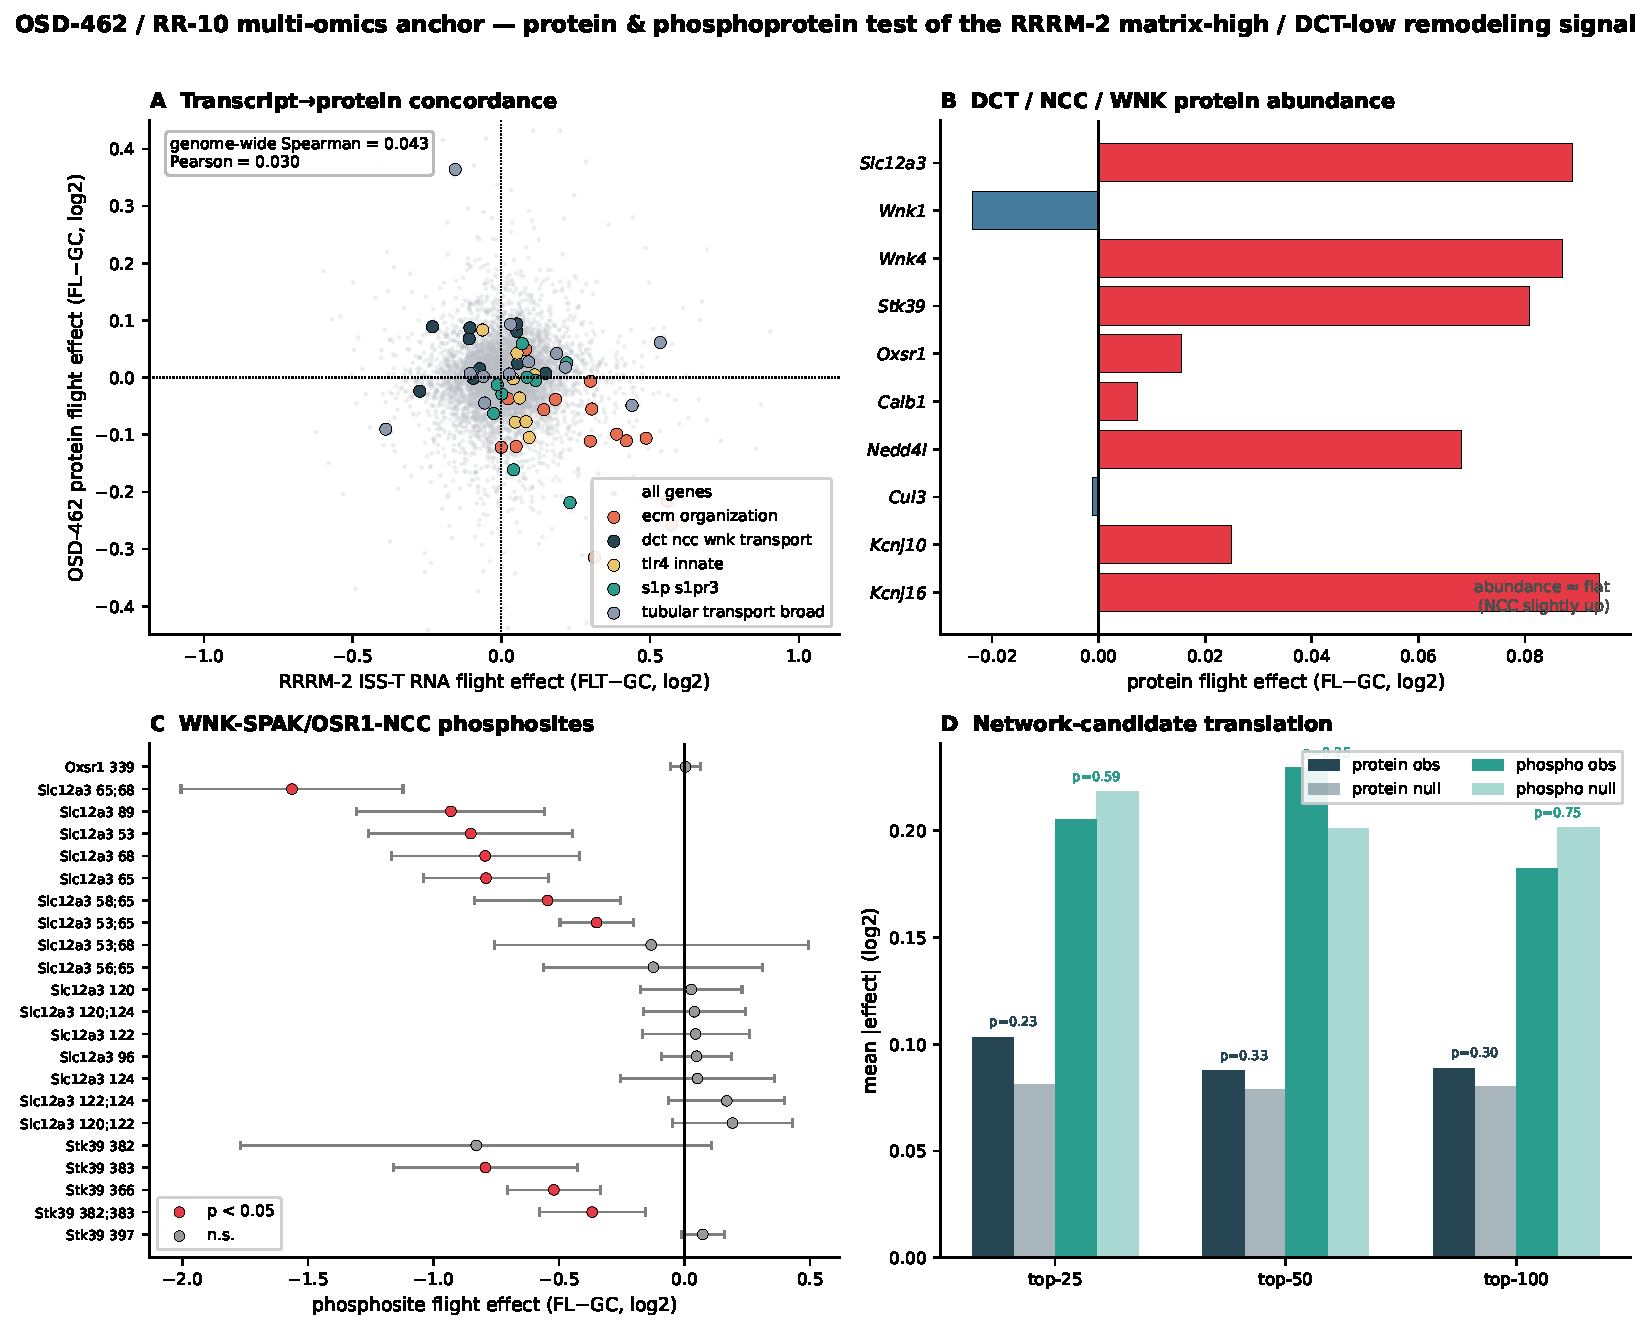
\includegraphics[width=\textwidth]{fig_osd462_multiomics_dashboard.pdf}
\caption{Multi-omics anchor dashboard. \textbf{A} Transcript (RRRM-2 ISS-T RNA) vs.\ OSD-462
protein flight effects; targeted sets coloured. Matrix genes (orange) occupy the
transcript-up / protein-down quadrant. \textbf{B} DCT/NCC/WNK protein abundances are flat
(NCC slightly up). \textbf{C} WNK--SPAK/OSR1--NCC phosphosite effects with 95\% CIs; the NCC
N-terminal cluster and SPAK activating sites (red, $p<0.05$) are strongly down while
C-terminal sites are flat. \textbf{D} Network-candidate translation: observed mean
$|$effect$|$ tracks the matched null at protein and phospho layers.}
\label{fig:dash}
\end{figure}

\begin{figure}[htbp]\centering
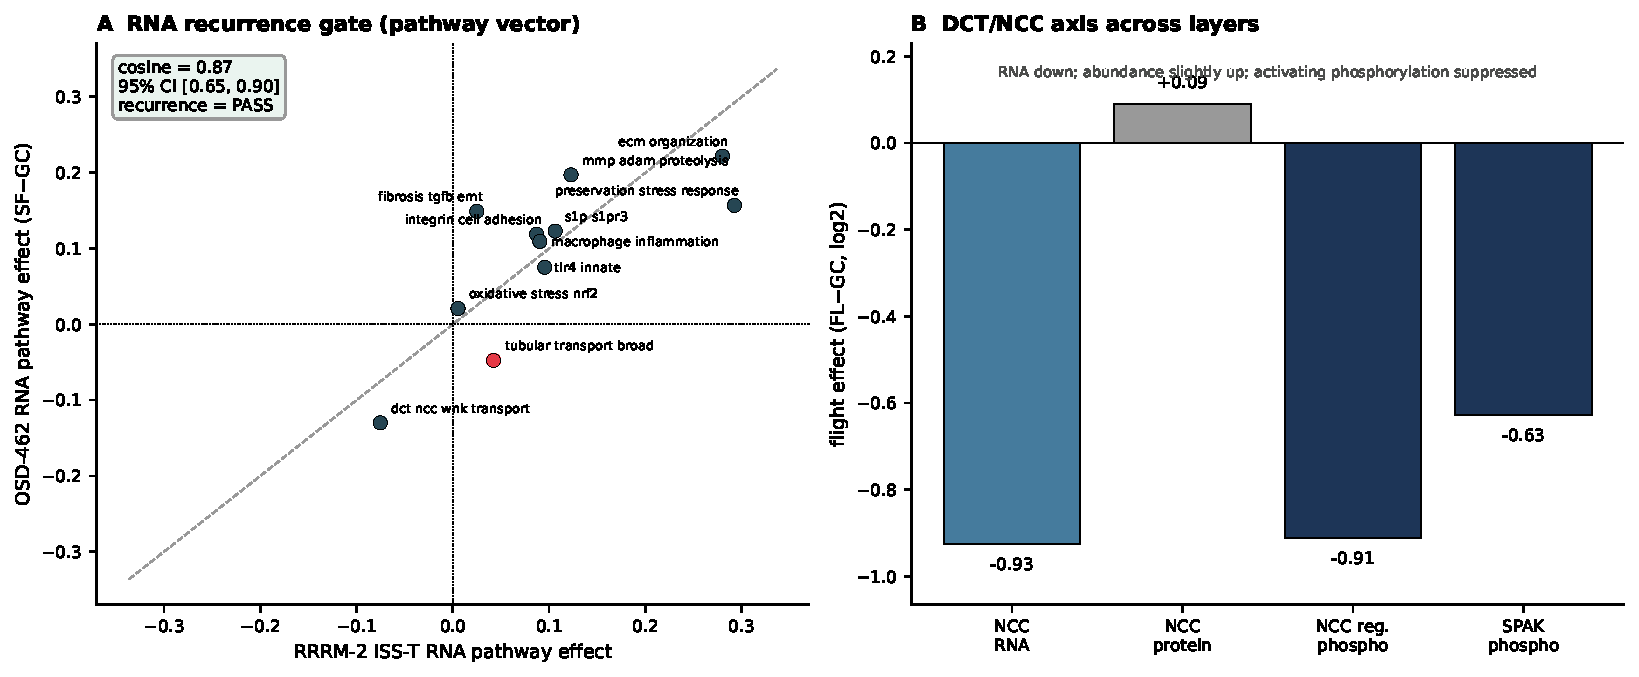
\includegraphics[width=\textwidth]{fig_osd462_rna_recurrence.pdf}
\caption{\textbf{A} RNA recurrence gate: OSD-462 vs.\ RRRM-2 pathway-effect vectors lie along
the identity line (cosine $0.87$, PASS); dct\_ncc\_wnk\_transport sits in
the shared-down quadrant, ECM/matrix in the shared-up quadrant. \textbf{B} The DCT/NCC axis
across layers: NCC transcript down, total NCC protein maintained, NCC regulatory
phosphorylation and SPAK phosphorylation strongly down --- an activity-level, not
abundance-level, change.}
\label{fig:recur}
\end{figure}

\section{Cross-layer integration and decision}
The pre-registered decision table resolves to: \emph{``Protein-abundance concordance NULL for both matrix and DCT; DCT signal relocates to the phospho/activity layer.''}
The honest reading across layers is two-pronged:
\begin{itemize}[leftmargin=1.4em]
\item \textbf{Matrix arm:} transcriptional only. The ECM program is induced at the RNA
level in both cohorts but matrix protein abundance is not increased (it is mildly,
significantly decreased), indicating transcript--protein uncoupling at terminal collection
rather than net matrix deposition.
\item \textbf{DCT/NCC arm:} an activity/signaling change. NCC transcript is down and total
NCC protein is preserved, but the SPAK$\to$NCC activating phosphorylation arm is specifically
suppressed. This both \emph{explains} why the DCT abundance test was null and \emph{upgrades}
the DCT claim to a signaling-level statement.
\end{itemize}

\section{Biological implications}
The WNK--SPAK/OSR1--NCC cascade is the master switch for Na--Cl reabsorption in the distal
convoluted tubule; phosphorylation of the NCC N-terminal threonines by SPAK/OSR1 is the
activating step, and SPAK is itself activated by WNK-dependent phosphorylation. Finding the
NCC activating cluster and the SPAK activating sites coordinately among the most
down-regulated phosphosites in the flight kidney --- with total NCC protein unchanged ---
is direct molecular evidence that spaceflight reduces NCC \emph{transport-pathway activation},
not transporter abundance. This is mechanistically more specific than the original
transcriptomic observation and connects to the physiological context that motivated the axis
(distal Na--Cl handling, K$^+$/Ca$^{2+}$ balance, volume regulation, and renal stone risk).
It also reframes the matrix result: the ``matrix-high'' signature is, in this cohort, a
transcriptional program not yet realised as protein, consistent with active remodeling
(transcription plus proteolysis) rather than fibrotic accumulation. Finally, the failure of
network-nominated candidates to translate cautions that LIONESS/node2vec rewiring scores
prioritise transcripts, not protein-level biology.

\section{What this can and cannot establish}
\textbf{Can:} that the RNA remodeling \emph{direction} reproduces in a second, independent,
cross-strain flight cohort at the RNA level; that the specific WNK--SPAK--NCC activation arm
is suppressed at the phosphoprotein level; and that matrix induction is transcript-level only.
\textbf{Cannot:} physiology. There is no histology and no urine/serum electrolyte data in
scope; even perfect concordance would yield a molecular claim (``reduced NCC
transport-pathway activation''), not a functional one (``kidney Na--Cl handling changed'').
A single terminal time point cannot resolve the transcript$\to$protein timing that would
explain the matrix uncoupling. The result does not rehabilitate ``network rewiring'' as a
mechanism-discovery method. Histology and urine/serum chemistry remain explicit future work.

\section{Reproducibility}
All numbers and tables in this document are generated directly from the analysis outputs
under \texttt{data/results/run\_20260521\_osd462\_anchor/osd462\_anchor/}: harmonized flight effects
(\texttt{osd462\_flight\_effects.tsv}), RNA recurrence
(\texttt{osd462\_rna\_recurrence.tsv}), protein concordance
(\texttt{protein\_concordance\_summary.tsv}), phospho axis
(\texttt{phospho\_axis\_summary.tsv}, \texttt{phospho\_axis\_verdict.tsv}), network
translation (\texttt{network\_translation.tsv}), and \texttt{results\_summary.json}. Each
layer writes a manifest with input SHA-256 digests; the run-level \texttt{manifest.json}
references them. Pipeline: \texttt{scripts/osd462/00\_harmonize.py} $\to$
\texttt{04\_rna\_recurrence.py} (gate) $\to$ \texttt{01\_protein\_concordance.py} $\to$
\texttt{02\_phospho\_axis.py} $\to$ \texttt{03\_network\_translation.py} $\to$
\texttt{05\_plot\_dashboard.py} $\to$ \texttt{06\_compile\_summary.py} $\to$
\texttt{07\_build\_compendium.py}; core estimators in
\texttt{src/multiomics/osd462\_anchor.py} with unit tests in
\texttt{tests/test\_osd462\_anchor.py}. Matched nulls use 10000 draws (seed 20260521);
the RNA recurrence bootstrap uses 2000 resamples.

\end{document}
